\documentclass[10pt]{article}
\usepackage{float}
\usepackage{listings}
\usepackage[french]{babel}
\usepackage[utf8x]{inputenc}
\usepackage{subcaption}
\usepackage{listings}
\usepackage{wrapfig}
\usepackage{color}
\usepackage{amsmath}
\usepackage{dsfont}
\usepackage{amsfonts}
\usepackage{hyperref}
\usepackage{mathtools}
\usepackage{graphicx}
\usepackage{caption}
\definecolor{dkgreen}{rgb}{0,0.6,0}
\definecolor{gray}{rgb}{0.5,0.5,0.5}
\definecolor{mauve}{rgb}{0.58,0,0.82}
\usepackage[table]{xcolor}
\usepackage{adjustbox}
\usepackage{multirow}
%opening
\definecolor{Gray}{gray}{0.85}




\lstset
{frame=tb,
	language=R,
	aboveskip=3mm,
	belowskip=3mm,
	showstringspaces=false,
	framexleftmargin=5mm,
	columns= fixed,
	numbers = left,
	basicstyle={\small\ttfamily},	
	numberstyle=\tiny\color{gray},
	keywordstyle=\color{blue},
	commentstyle=\color{dkgreen},
	stringstyle=\color{mauve},
	breaklines=true,
	breakatwhitespace=true,
	tabsize=3
}


\title{
	\normalfont \normalsize 
	\textsc{Université de Technologie de Compiègne\\ 
		SY09:Analyse des données et Data-Mining , P17} \\
	[10pt]
	\rule{\linewidth}{0.5pt} \\[6pt] 
	\huge Rendu TP3\\
	\rule{\linewidth}{2pt}  \\[10pt]
}
\author{Zineb Slam, Oumaima Talouka}
\date{\normalsize \today}

\begin{document}
	{\let\newpage\relax\maketitle}	
	
		\begin{abstract}
			Dans de TP4 nous allons étudier 5 techniques de discriminante: l'analyse discriminante linéaire, l'analyse discriminante quadratique, le bayésien naive, la régression logistique et la régression logistique quadratique. 
		\end{abstract}
	


\section{Programmation}
\section{Application}
\subsection{Test sur données simulées}
Pour separer nos donnees en ensemble d'apprentissage et de test nous faisons de la sorte:
\begin{lstlisting}
train   = sample(1:n, round(2*n/3)) 
Xapp    = X[train, ]
zapp    = z[train]
Xtst  = X[-train, ]
ztst  = z[-train]
\end{lstlisting}
\subsubsection{Syhn2-1000}
Dans ce qui suit nous avons représenté les résultats de calcul de l'erreur de test dans les données Synth2-1000. Les graphes sont représentés ci-dessous avec les frontières de décisions et les erreurs pour chaque classifieur.

\begin{minipage}{.5\textwidth}
	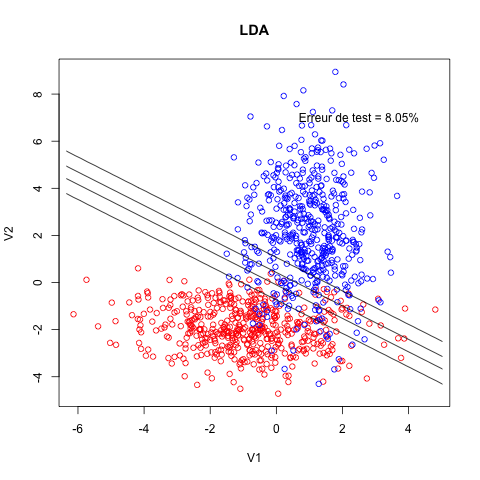
\includegraphics[width=45mm]{Figures/synth2_lda.png}
\end{minipage}%
\hspace{0.02\linewidth}
\begin{minipage}{.5\textwidth}
	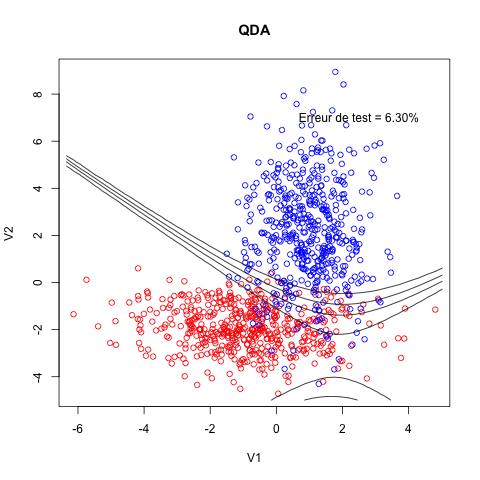
\includegraphics[width=45mm]{Figures/synth2_qda.png}
\end{minipage}

\begin{center}
	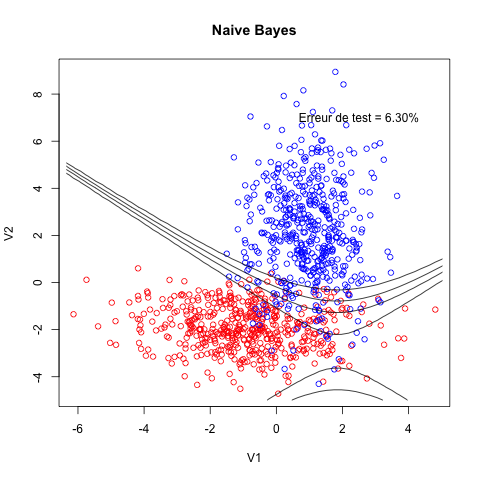
\includegraphics[width=45mm]{Figures/synth2_nb.png}
\end{center}
\begin{minipage}{.5\textwidth}
	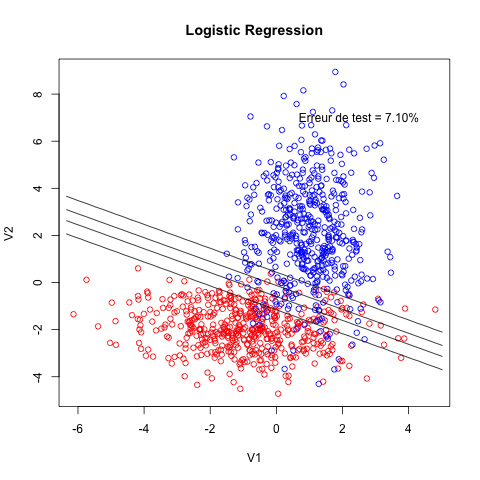
\includegraphics[width=45mm]{Figures/synth2_logreg.png}
\end{minipage}%
\hspace{0.02\linewidth}
\begin{minipage}{.5\textwidth}
	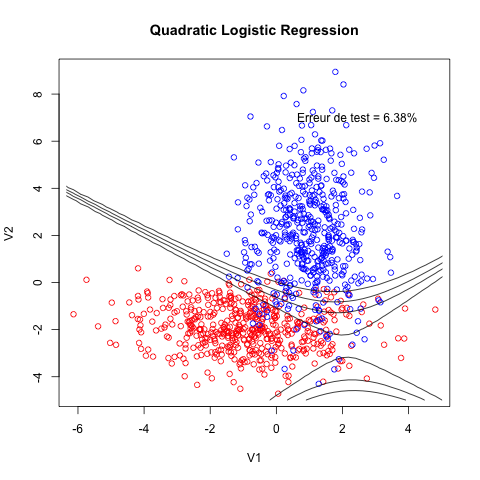
\includegraphics[width=45mm]{Figures/synth2_logregquad.png}
\end{minipage}


On remarque que l'erreur de test est inférieur a  9\% pour tous les classifieurs. Selon la représentation des points on remarque que les classes ont a peu pres la même distribution et on n'a qu'une dizaine de  points qui sont confondus entre les 2 classes. Par conséquent les classes peuvent être  linéairement séparés, ceci est illustre par l'erreur de test puisqu'on voit que la regression quadratique n'apporte qu'une légère amélioration de l'ordre de 1\%.
Neanmois il faut remarquer que le classifieur Bayésien Naïve performe aussi bien que les régressions quadratiques. Ceci était prévisible vu que nos classes sont orientes vers les axes du plan et ... Ainsi il est plus intéressant dans ce cas d'utiliser le classifieur Bayésien Naïve vu qu'on n'estime que paramétrés au lieu de avec la régression quadratique ou même la logistique quadratique.


\subsubsection{Synth3-1000}
Nous nous intéressons a présent aux données de Synth3-1000 avec 1000 individus.

\begin{minipage}{.5\textwidth}
	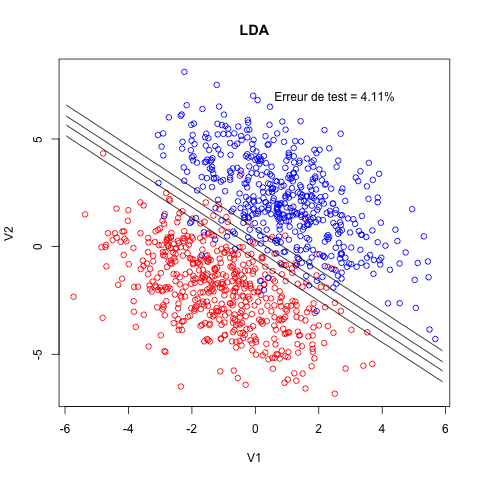
\includegraphics[width=45mm]{Figures/synth3_lda.png}
\end{minipage}%
\hspace{0.02\linewidth}
\begin{minipage}{.5\textwidth}
	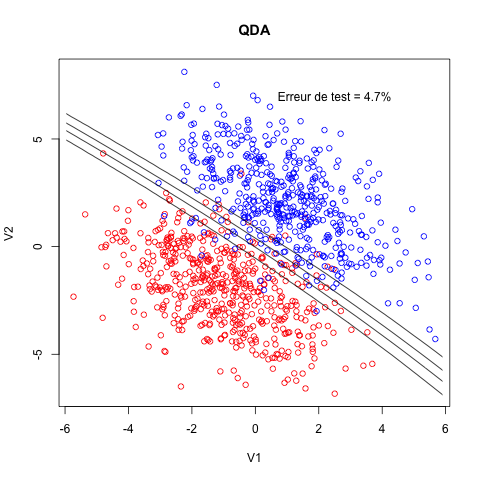
\includegraphics[width=45mm]{Figures/synth3_qda.png}
\end{minipage}

\begin{center}
	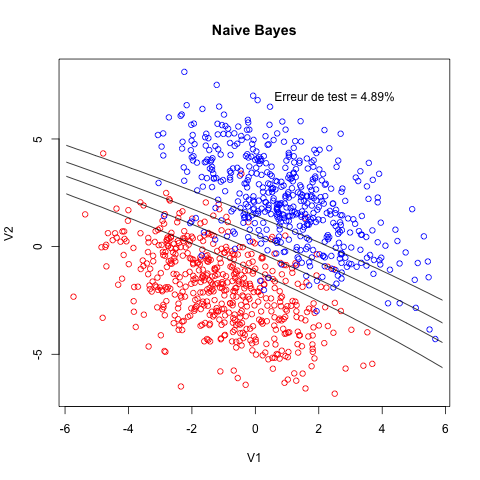
\includegraphics[width=45mm]{Figures/synth3_nb.png}
\end{center}
\begin{minipage}{.5\textwidth}
	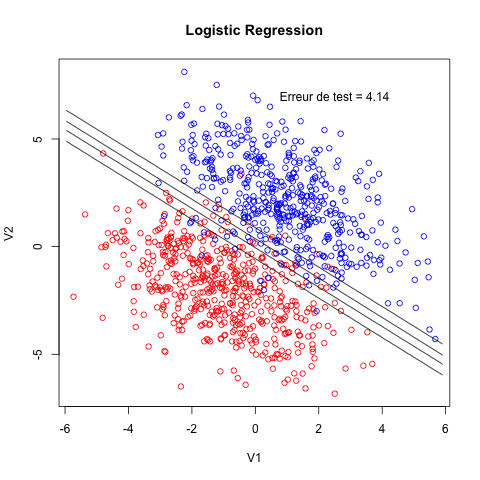
\includegraphics[width=45mm]{Figures/synth3_logreg.png}
\end{minipage}%
\hspace{0.02\linewidth}
\begin{minipage}{.5\textwidth}
	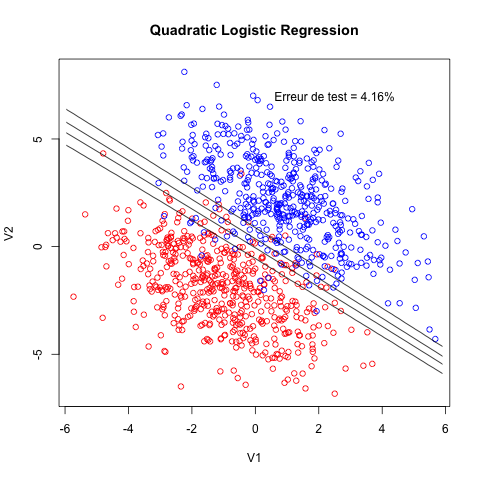
\includegraphics[width=45mm]{Figures/synth3_logregquad.png}
\end{minipage}

On remarque en représentant les données que les classes ont les même orientation et distributions, et peuvent êtres linéairement séparés.  Il est donc normal de voir que les erreurs de test du LDA  sont faibles et que celles ci sont approximativement égales a celles du QDA. 




\subsection{Test sur données réelles}
\subsection{Pima}
\subsection{Breast Cancer}
\subsubsection{Description des données}
Avant de se lancer dans l'analyse de données, nous allons essayer de décrire ces données pour mieux analyses les résultats obtenus. Breast Cancer Winsconsin compte 683 individus et 9 variables quantitatives explicatives.
\subsubsection{Analyse discriminantes}
Le tableau ci-dessous montrent les résultats obtenus avec les différentes méthodes d'analyses discriminantes.
\begin{center}
	\begin{tabular}{|c | c | c| c| }
		\hline
	LDA & QDA & Naive Bayes & Log Reg \\
	\hline	
	4.57\% & 5.03\% & 3.98\% & 4.02\%
	\end{tabular}
\end{center}

Contrairement aux résultats obtenus dans les données de \textit{Synth} on remarque ici que les performances des classifieurs diffèrent. En effet le classifieur Bayésien Naïf et la régression logistique sont ceux qui classent au mieux nos données suivi par la methode d'analyse discriminante linéaire et quadratique. 
La methode la plus performante ici est le  classifieur Bayésien Naïf. En effet si on s'intéresse a la matrice de variance  on remarque que les valeurs dans la diagonale sont les plus grandes. La matrice est donc quasi-diagonale. Ce qui vérifie l'hypothèse d'indépendance des données du classifieur Bayésien Naïf. \\
La methode d'analyse linéaire n'est pas aussi performante bien car si on observe les matrice de variances de chaque classe on remarque que l'hypothèse d'homoscédasticité n'est pas vérifiée.

\subsubsection{Conclusion}
On remarque que dans les 3 cas la régression logistique fournir le pourcentage d'erreur le plus faible. Néanmoins cette méthode est trop couteuse quant aux nombre de paramètre a estimer. Remarquons qu'appliquer la la méthode de régression logistique quadratique aurait été trop couteux dans ce cas ou on a 8 variables d'une part. 

\subsubsection{Arbres de décisions}
Pour obtenir l'arbre de décision de l'ensemble d'apprentissage nous utilisons la fonction \textit{tree} du \textit{package tree}. Nous fixons les paramètres\\  \textit{control=tree.control(nobs=dim(Dapp)[1],mindev = 0.0001)}  comme demandé dans ce TP. \textit{nobs} est le nombre d'observations des données d'apprentissage , \textit{mindev} est la deviance entre les noeuds. Si mindev=0 il essaye de fit parfaitement les données. La fixation de ces paramètres influence directement la taille (le nombre de nœuds) de l'arbre.\\
\begin{minipage}{.5\textwidth}
	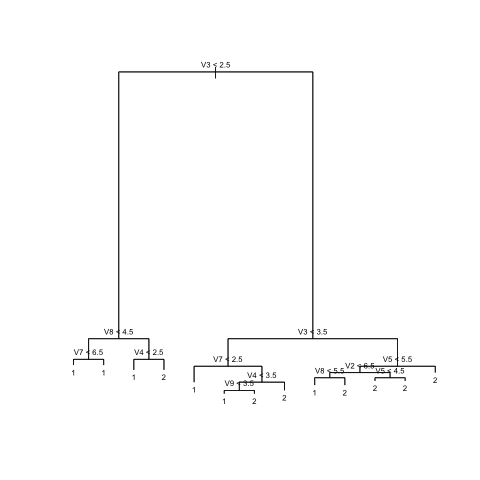
\includegraphics[width=50mm]{Figures/bcw_apptree.png}
\end{minipage}%
\hspace{0.001\linewidth}
\begin{minipage}{.5\textwidth}
	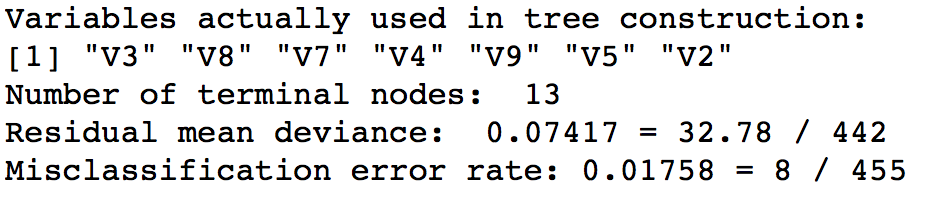
\includegraphics[width=65mm]{Figures/bcw_apptree_summary.png}
\end{minipage}

Ainsi sur l'ensemble d'apprentissage on a une erreur de mal classement de 1.76\%. On remarque ici V3, V8, V7, V8, V9, V5 et V2. La  complexité d'un arbre est évaluée avec le nombre de feuilles qu'il a puisque se sont les différentes classes. Ainsi la fonction \textbf{tree} nous retourne un arbre avec 13 nœuds et donc 13 partitions.\\
Nous allons a présent utiliser la méthode de cross validation pour trouver l'hauteur optimale de l'arbre. On utilise la fonction R \textbf{tree.cv} avec k=10 pour faire une \textit{10-fold cross validation}, qui consiste a diviser l'ensemble d'apprentissage en 10 ensembles et utiliser un a chaque fois comme ensemble de validation.  Les résultats sont représentés ci-dessous sous forme du graphe de l'évolution du nombre d'individus mal classes en fonction de la 

\begin{minipage}{.4\textwidth}
	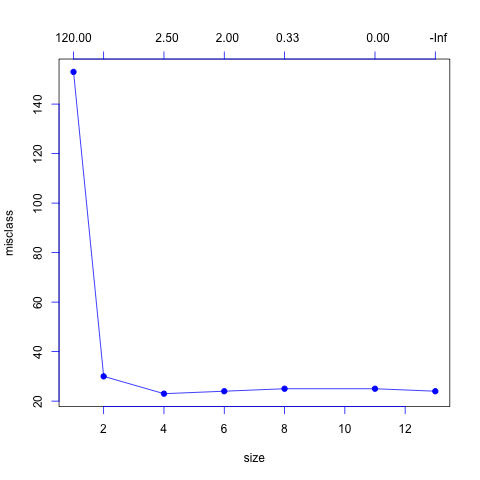
\includegraphics[width=45mm]{Figures/bcw_cvplot.png}
		\captionof{figure}{Graphe de l'evolution des individus mal-classes en fonction du nombre de feuilles}
\end{minipage}%
\hspace{0.01\linewidth}
\begin{minipage}{.65\textwidth}
 \begin{lstlisting}
min= which(bcw.cv$dev==min(bcw.cv$dev))
best.size= bcw.cv$size[min]
 \end{lstlisting}
\end{minipage}
On récupère donc la taille de l'arbre qui minimise l'erreur (le nombre d'individus mal classes) qui est 4. Ensuite on utilise la fonction\textbf{prune.misclass}permet d’élaguer l’arbre en mettant 4 comme taille de l'arbre. Grâce a la fonction \textbf{predict} on obtient en sortie le vecteur de prédiction de classes. La matrice ci-dessous est la matrice de confusion des vrais classement et des prédictions.
\begin{minipage}{.5\textwidth}
	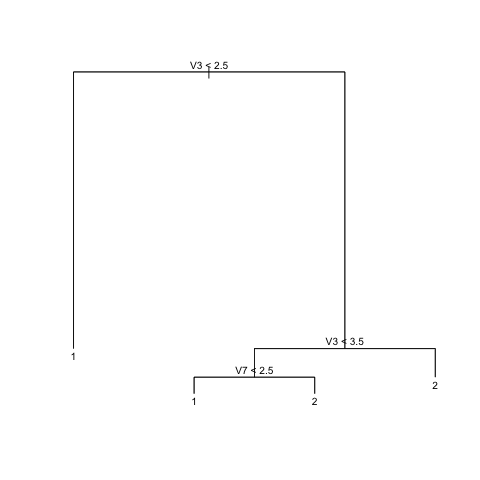
\includegraphics[width=45mm]{Figures/bcw_prunedtree.png}
\end{minipage}%
\hspace{0.00\linewidth}
\begin{minipage}{.4\textwidth}
\begin{tabular}{c  c c}
  & 1  &  2 \\
1 & 135 &   7 \\
2 &  6&  80
\end{tabular}
\end{minipage}

Nous utilisons ensuite les instructions pour calculer l'erreur de test:
\begin{lstlisting}
tree.pred = predict(bcw.cv.pruned, Xtst, type = "class")
res = with(Xtst, table(tree.pred, ztst))
error.test = res[1,2] + res[2,1] / nrow(Xtst)
print(paste("Test Error  ",error.test))
\end{lstlisting}

Nous obtenons 6.03\% comme erreur de test.




\section{Spams challenge}
\end{document}